\subsection{General overview of a \acrshort{csac}}
\label{subsec:general_overview}

Before proceeding analyzing in detail the components of a \acrshort{csac}, it's important to understand the general idea that governs its operation.

With respect to traditional quartz oscillators, \acrshort{csacs} exploit the use of a close loop control system to stabilize the frequency of the local oscillator to the atomic transition frequency.
In other words, \acrshort{csacs} leverage the intrinsic stability of atomic transitions to discipline an oscillating circuit based on a vibrating quartz crystal.
Many of the instabilities that affect traditional oscillators, such as temperature sensitivity, aging, and vibration sensitivity (common in classical quartz oscillators), are mitigated by the use of atomic transitions that by their nature are more stable and less sensitive to external factors.

\paragraph{The Building Blocks}

From a functional perspective, a \acrshort{csac} can be broken down into four main blocks, each with a specific role in the system:

\begin{itemize}
    \item \acrfull{pp}: it can be considered the heart of the clock. It contains an atomic vapor cell where the atomic excitation and interrogation take place.
    \item \acrfull{cl}: it can be considered the brain of the \acrshort{csac}. It constantly analyzes signals from the physics package and uses this information to fine-tune the frequency of the local oscillator.
    \item \acrfull{lo}: it's the effective source of the clock. Given its intrinsic instability, it's constantly disciplined by the control loop to block its frequency to a known multiple of the atomic transition frequency.
\end{itemize}

Notice that a fourth block is also present in the system, that is the Frequency Synthesizer (FS), which takes the LO's frequency and multiplies it by a known factor to match the range of frequencies needed to interact with the atoms within the physics package.
For the sake of simplicity, we will not delve into the details of the FS in this section, limiting our analysis to the PP, CL, and LO.

The mentioned components are arranged in a closed-loop system, as illustrated in Figure \ref{fig:CSAC-general-overview}.

\begin{figure}[H]
    \centering
    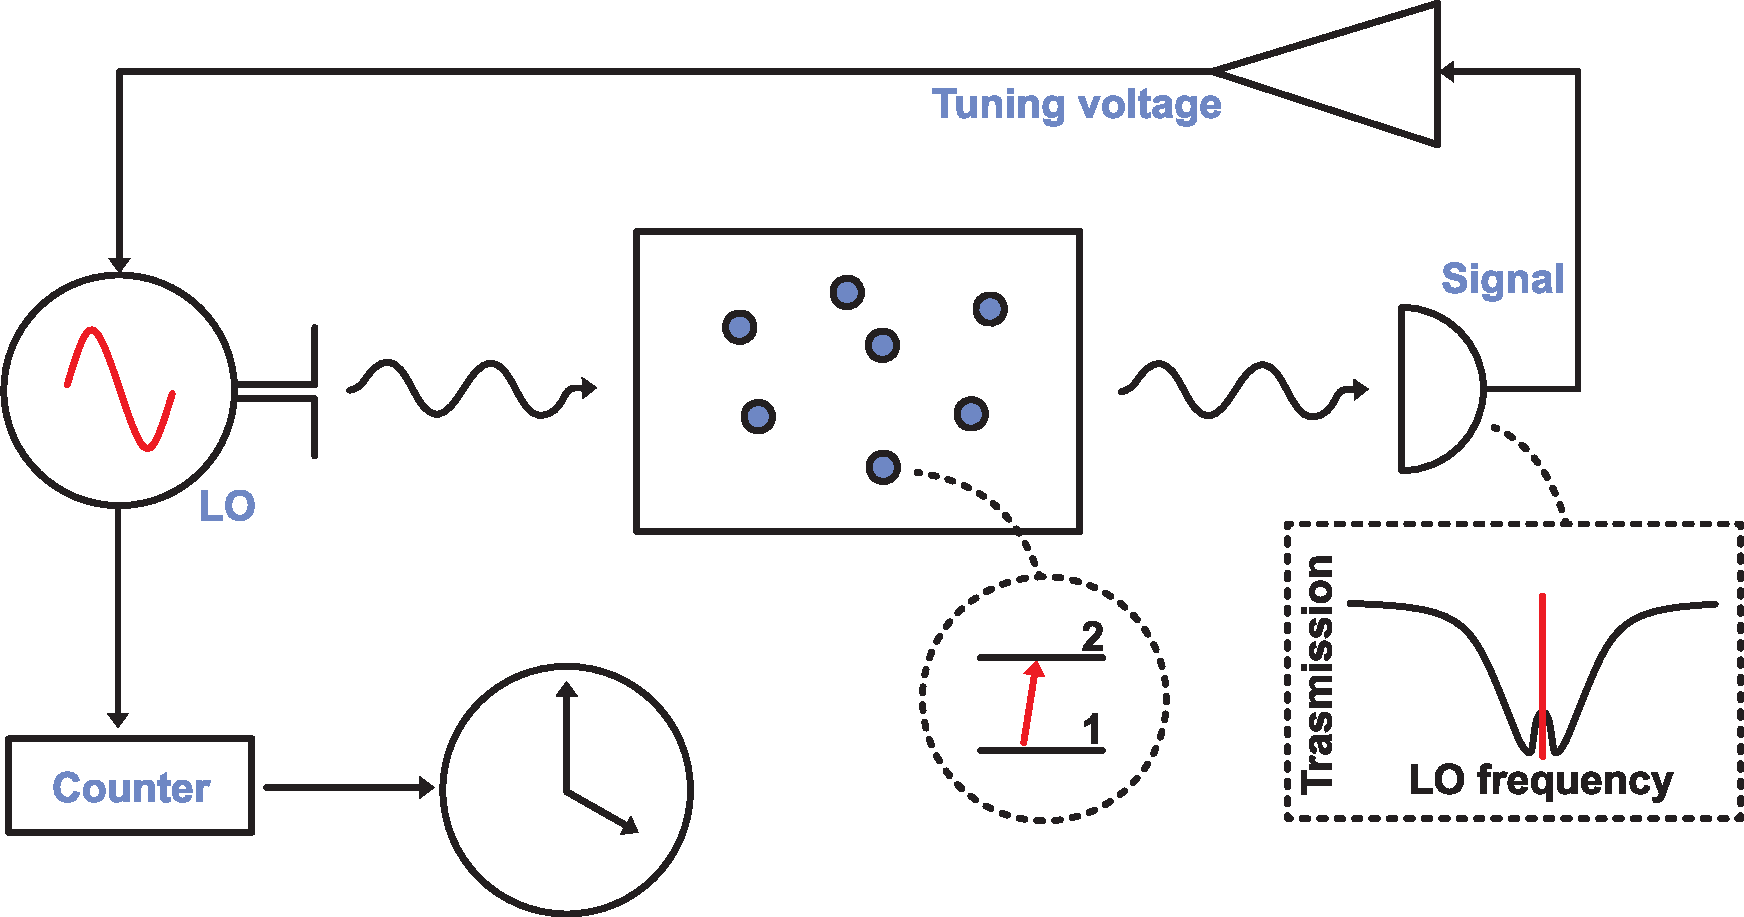
\includegraphics[width=0.7\textwidth, max width=\linewidth]{pdf/CSAC-scheme.pdf}
    \caption{General overview of a \acrshort{csac}}
    \label{fig:CSAC-general-overview}
\end{figure}

In the following sections, we will go through each main block of the \acrshort{csac}, highlighting their fundamental physics, understanding their role in the general framework of the clock, and identifying potential limitation that affect the overall performance.
